\documentclass[tikz,border=4pt]{standalone}
\usepackage{amsmath,amssymb}
\usetikzlibrary{positioning,arrows.meta,calc,fit}
\begin{document}
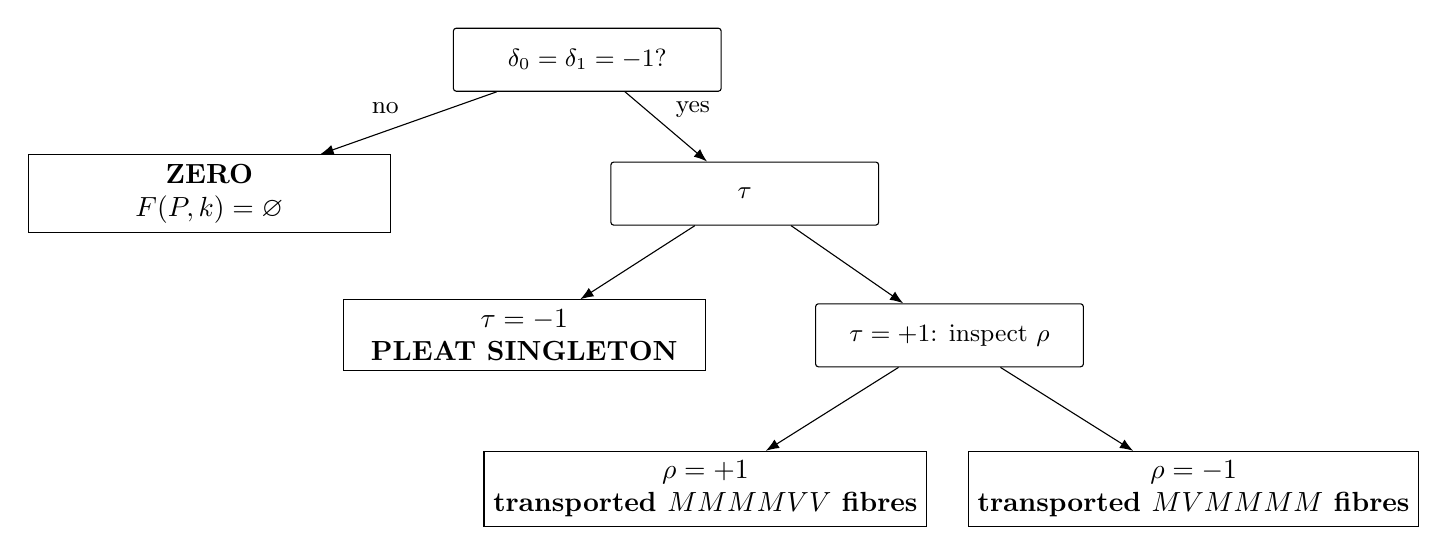
\begin{tikzpicture}[
  font=\small,>=Latex,
  q/.style={draw,rounded corners=1pt,align=center,minimum width=34mm,minimum height=8mm},
  leaf/.style={draw,align=center,minimum width=46mm,minimum height=9mm,font=\bfseries}
]
\node[q] (d) at (0,0) {$\delta_0=\delta_1=-1$?};
\node[leaf] (zero) at (-4.8,-1.7) {ZERO\\$F(P,k)=\varnothing$};
\node[q] (tau) at (2.0,-1.7) {$\tau$};
\node[leaf] (pleat) at (-.8,-3.5) {$\tau=-1$\\PLEAT SINGLETON};
\node[q] (rho) at (4.6,-3.5) {$\tau=+1$: inspect $\rho$};
\node[leaf] (plus) at (1.5,-5.45) {$\rho=+1$\\transported $MMMMVV$ fibres};
\node[leaf] (minus) at (7.7,-5.45) {$\rho=-1$\\transported $MVMMMM$ fibres};
\draw[->] (d) -- node[above left] {no} (zero);
\draw[->] (d) -- node[above right] {yes} (tau);
\draw[->] (tau) -- (pleat);
\draw[->] (tau) -- (rho);
\draw[->] (rho) -- (plus);
\draw[->] (rho) -- (minus);
\end{tikzpicture}
\end{document}
